\chapter{Introduction to R}

\section*{}

R is a high-level programming language and environment for statistical computing and graphics. For many years, R has belonged to the most popular programming languages, especially in the machine learning community. It is primarily
focused on statistical operations, working with vectors and matrices, creating
statistical models on a few lines, etc. \cite{ref209}.

R provides facilities for effective data handling and storage, operators for
calculations on multidimensional data, a collection of tools for data analysis and
graphical facilities for data analysis and display. It also includes a simple and
effective programming language which includes all common elements of programming languages, such as branchings, loops, user-defined functions, or input
and output facilities \cite{ref117}. The capabilities of R language can be augmented with
compiled code written in C, C++, or Fortran \cite{ref80}.

The language, created by Ross Ihaka and Robert Gentleman at the University of Auckland more than twenty years ago, has derived its syntax, semantics,
and implementation from two other older languages – S and Scheme \cite{ref125}. R
is an open-source project, which means that you can see how the functionality
is implemented and modify what does not work exactly according to your requirements \cite{ref203}. R is very popular in science, engineering, and education, with
many active communities. The R Foundation supports the R project and its development, organizes conferences, and patronizes the R Journal (\textit{\href{https://journal.r-project.org/}{https://journal.rproject.org}}).

This book does not want to provide exhaustive information on programming
in R. The language is used here as one of many options with the aim of demonstrating the principles of machine learning algorithms and getting real results
from analyzing texts. An interested reader can refer to an endless resource of
books (e.g., \textit{The R Primer} by C. T. Ekstrom {CRC Press}, \textit{R in a Nutshell: A Desktop Quick Reference} by J. Adler {O’Reilly}, The R Book by M. J. Crawley
{Wiley}, or \textit{The Art of R Programming: A Tour of Statistical Software Design}
by N. Matloff {No Starch Press}. Probably the most compete information can be
found in \textit{The R Manuals available at \href{https://cran.r-project.org/}{https://cran.r-project.org/manuals.html}}.

Some of the tasks can be achieved with core R functions and capabilities,
some other algorithms are implemented by various packages available in the
\textit{Comprehensive R Archive Network} (CRAN). The archive currently contains almost 14,000 packages solving problems from various domains and uploaded by
many authors. To solve one specific task, multiple packages are often available.
In this book, we do not consider all possible options as the main focus is not
on R but the machine learning algorithms. Also only the necessary functionality (only some functions and their parameters) of the packages is used, which is
sometimes only a small fraction of the package capabilities. The complete functionality and parametrization of algorithms can be always found in the package
documentation.

\section{Installing R}
We assume that you have a PC or an Apple Mac and you want to install R on the
hard disc and that you have access to the Internet. The R language is available
as free software under the terms of the Free Software Foundation’s GNU General Public License (\textit{\href{https://www.gnu.org/}{https://www.gnu.org}}) in source code form at \textit{\href{https://www.r-project.org/}{https://www.rproject.org}}. It can be compiled and run on a wide variety of UNIX platforms, as
well as on Windows and Mac OS X.

In order to get a current version of the language, go to the CRAN site
(\textit{\href{https://cran.r-project.org/}{https://cran.r-project.org/mirrors.html}}) and choose your preferred CRAN mirror. Then, you can decide the platform (Linux, Max OS X, or Windows) for
which to obtain a precompiled binary distribution. You can also get the source
code for all platforms (see Figure 2.1).

In our example, a version for the Windows operating system will be installed.
The installation process for all other supported systems is described on the website of the R project.

There exist a few possibilities of the R download for Windows. The base
sub-directory is preferred for the first installation.

While older distributions are still accessible, the newest distribution is recommended for downloading. The executable distribution file (e.g., \textit{R-3.5.1-win.exe})
can be easily downloaded and run. R will be installed in an ordinary process with
the assistance of an installation wizard.

\begin{figure}[!ht]
    \centering
    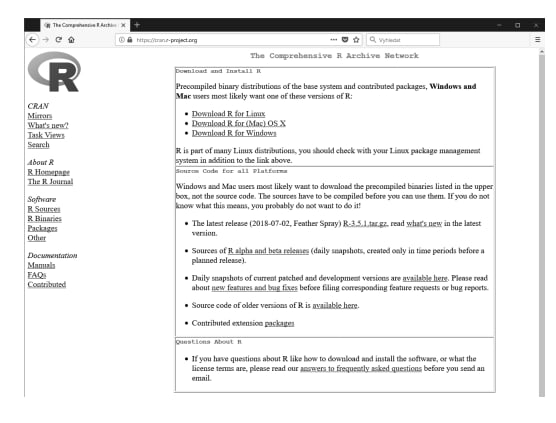
\includegraphics[width = \textwidth]{chapter/chapter2/figure2.1.jpg}
    \caption{The home page of the R project.}
    \label{fig:placeholder2}
\end{figure}

\section{Running R}

To run R under Windows, just click on the R icon. A graphical user interface, as
in Figure 2.2, will be displayed.

Inside the R graphical user interface, you can see a menu, toolbar, and R
Console. In the console, below the header (a version of R and some initial information about the system) you will see a line with a > symbol on the left.
This is called a prompt and this is where you type your commands. Try to enter
citation() to see how to cite the R software in your work.

An easier way to use R is by using some of the integrated development environments (IDE). A list of some R IDEs includes:

\begin{itemize}
    \item R Studio,
    \item Visual Studio for R,
    \item Eclipse,
    \item Red-R,
    \item Rattle,
    \item and many others.
\end{itemize}

\begin{figure}[!ht]
    \centering
    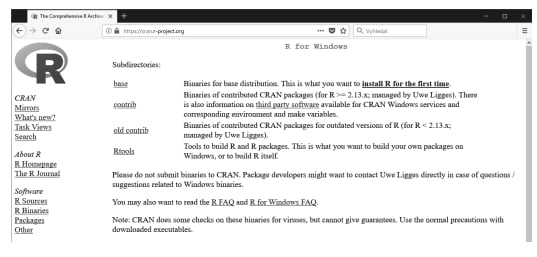
\includegraphics[width = \textwidth]{chapter/chapter2/figure2.2.jpg}
    \caption{Selecting a subdirectory for R installation.}
    \label{fig:placeholder3}
\end{figure}

\begin{figure}[!ht]
    \centering
    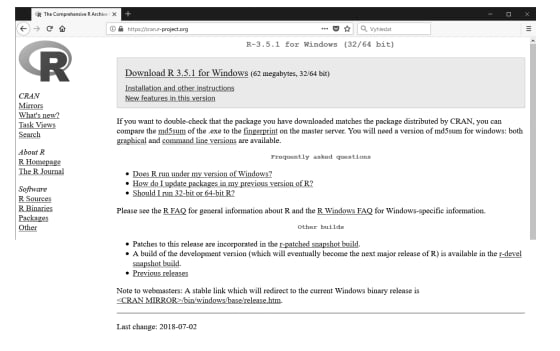
\includegraphics[width = \textwidth]{chapter/chapter2/figure2.3.jpg}
    \caption{Getting the newest R package.}
    \label{fig:placeholder4}
\end{figure}

\textit{RStudio} has been voted the most popular R IDE by the readers of KDnuggets \textsuperscript{1}. Thus, in the following text, we are using RStudio for the examples.

\footnote{\href{https://www.kdnuggets.com/polls/2011/ir-gui-used.html}{https://www.kdnuggets.com/polls/2011/ir-gui-used.html}}

\begin{figure}[!ht]
    \centering
    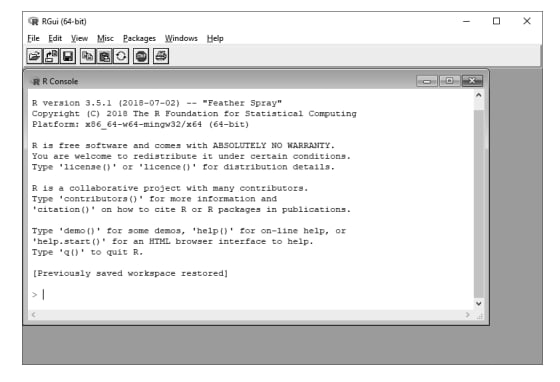
\includegraphics[width = \textwidth]{chapter/chapter2/figure2.4.jpg}
    \caption{The graphical user interface of the R system on Windows.}
    \label{fig:placeholder5}
\end{figure}

\section{RStudio}

RStudio is an IDE for R available in open source and commercial editions. It
enables syntax highlighting, code completion, and smart indentation when writing the code that can be executed directly from the source editor. It facilitates
the work of programmers by providing facilities like jumping to function definitions, integrated documentation and help, managing multiple working directories, multiple-file editing, interactive debugger for diagnosing and fixing errors,
and package development tools.

RStudio can be run on various operating systems like Windows, Mac OS
X, and Linux. It is a very useful and powerful tool for programming in R. We
suggest that readers use RStudio when learning from this book. To get RStudio,
go to \textit{\href{https://posit.co/}{https://www.rstudio.com/}} and follow the instructions.

On launching RStudio, the following panes are displayed (see Figure 2.5):

\begin{itemize}
    \item \textit{Console} where R commands/scripts can be executed and \textit{Terminal} allowing the access to the system shell (top left-hand corner of the screen)

    \item \textit{Environment} and \textit{History}, and \textit{Connections} – information about environment, history of commands, and connections to external data sources (top
right-hand corner of the screen)
\end{itemize}

\begin{figure}[!ht]
    \centering
    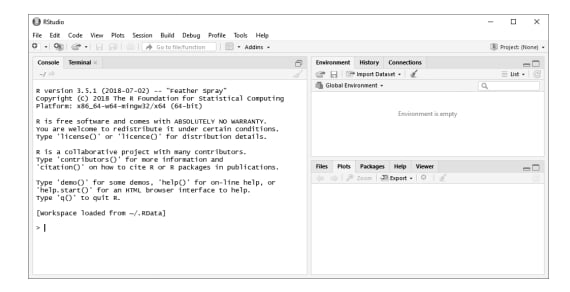
\includegraphics[width = \textwidth]{chapter/chapter2/figure2.5.jpg}
    \caption{The graphical user interface of RStudio}
    \label{fig:placeholder6}
\end{figure}

\begin{itemize}
    \item \textit{Files} in the current working directory, installed R \textit{packages, plots, a help}
display screen, and a \textit{viewer} of local web content (bottom right of the
screen).
\end{itemize}

A new script, i.e., a code that can be saved on a disk and later reopened or
executed, can be created by choosing \textit{File / New File / RScript} in the main menu.
A new empty editor window, ready for editing, will appear.

It is always good practice to choose a working directory when programming
in RStudio. The working directory is a folder where you store your R code, figures, etc. To set the working directory, go to \textit{Session / Set Working Directory /
Choose Directory} in the main menu.

\subsection{Projects}

RStudio provides a very useful feature known as \textit{Projects} to organise your work
into meaningful contexts. A project puts together R scripts, input data, analytical
results, or plots, and has its own working directory, history, or workspace.

A new project can be created by selection of \textit{File / New Project} in the main
menu. A project can be started in a new directory, associated with an existing
working directory, or cloned from a version control (Git or Subversion) repository.

Select the New Directory option, then \textit{New Project}, choose a name for your
project directory, and select its location. A new directory will be created, together
with a project file (with the .\textit{Rproj} extension) and a hidden directory .\textit{Rproj.user}
with project-specific temporary files project. The will be loaded in RStudio and
its icon displayed to the right of the toolbar. RStudio will also automatically set
the working directory to the project directory.

\begin{figure}[!ht]
    \centering
    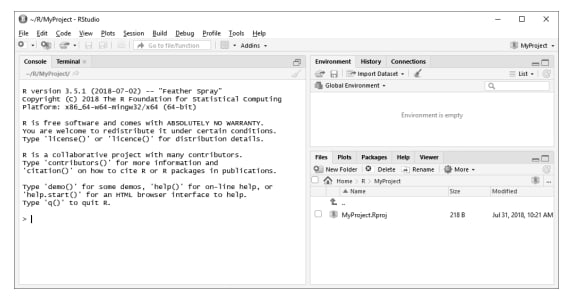
\includegraphics[width = \textwidth]{chapter/chapter2/figure2.6.jpg}
    \caption{A new project created in RStudio.}
    \label{fig:placeholder7}
\end{figure}

\subsection{Getting Help}\

Help pages for a desired object (e.g., operator or function) are invoked by the
help() function. The name of an object for which help should be displayed is
passed as a string parameter (enclosed in single or double quotes). However, a
shortcut ? is often used (quotation marks not necessary). For example, typing
?sin opens a help page containing a documentation for the sin() function.

If you do not remember the precise name of the object but know the domain to which it is related (e.g., trigonometric functions in this case) use the
help.search() function. A string passed to the function will be searched
for in the documentation and the possibilities associated with this query
will be displayed. The same can be achieved with the ?? shorthand (e.g.,
??trigonometric or ??"trigonometric functions").

Another way to get help in RStudio is to select \textit{Help / R Help} in the main
menu or by going to the Help pane and browsing the manual pages or searching
for a specific answer using the search capability.

To see some examples related to, for instance, a function, use the
example() function, where the appropriate name is passed as a parameter (e.g.,
example(help) or example(‘+’)).

\section{Writing and Executing Commands}

When R is ready to accept commands (expressions, consisting of objects and
functions) from a user, the R console displays a > prompt. After it receives a
command (something is typed on the

\begin{figure}[!ht]
    \centering
    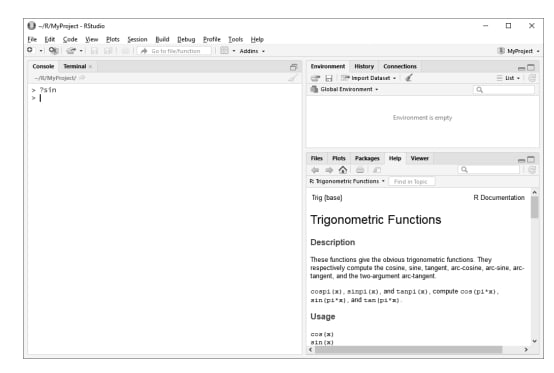
\includegraphics[width = \textwidth]{chapter/chapter2/figure2.7.jpg}
    \caption{Displaying a help for an existing function.}
    \label{fig:placeholder8}
\end{figure}

\hspace{-1.5em}keyboard and Enter is pressed) R tries to
execute it. Subsequently, a result is shown2
in case of a successful execution and
a new > prompt is displayed again.

\begin{verbatim}
> 3+8/4 # after writing the expression, Enter was pressed
[1] 5
> "Hello, World!"
[1] "Hello, World!"
\end{verbatim}

When the command is not complete (for example, a closing parenthesis,
quote, or operand is missing) R will submit a request to finish it. The console
will now display a + prompt. The user can complete the command and the result will then be displayed. To finish writing the command when the + prompt is
displayed, just press \textit{Esc}.

\footnote{%
The number in square brackets is related to numbering the elements of the output and can be ignored. 
Here, for example, the output is a vector and the row starts with its first element.%
}

\begin{verbatim}
> 5+ # Enter was pressed here
+ 6 # Enter was pressed here
[1] 11
> 5+ # Enter was pressed here
+ # Esc was pressed here

>
\end{verbatim}

Two or more expressions can be placed on a single line. In that case they must
be separated by semicolons with optional white spaces:

\begin{verbatim}
> 1+2;2-3; 4/5
[1] 3
[1] -1
[1] 0.8

\end{verbatim}

To complete a piece of code, press \textit{Tab}. A list of possible completion options
(together with their short descriptions when applicable) that fit the given part of
code is displayed (RStudio analyzes the code to suggest only meaningful options). By selecting one of them, the selected piece of text will be inserted to a
command. If there exists only one possibility of what can be inserted no options
are displayed and the code is completed immediately.

By pressing the up and down arrow keys, previously entered commands can
be accessed. Pressing \textit{Ctrl+Up} displays the list of all commands. They are also
accessible in the History pane of RStudio.

Comments are useful pieces of the code that help programmers explain what
various part of the code mean. They are completely ignored by the R interpreter.
A comment starts with the symbol \#. The subsequent characters until the end of
line are the comment. R does not allow comments running into multiple lines.
To overcome this problem, a quoted string occupying more than one line can be
used. The string will be evaluated as normal but will not perform any action.

\section{Variables and Data Types}

To store and access values in computer memory, so called ‘objects’ are used. Objects are data structures containing values of a certain type. Every such a structure
might have a class attribute, which determines the class of the object, associated
to it. If such an attribute does not exist, it will be computed from the type of the
values stored in the object.

There exist a few atomic (single-valued) data types (classes, returned by the
\texttt{class()} function as mentioned below) that are typically used in machine learning:

\begin{itemize}
    \item character
    \item numeric
    \item integer
    \item logical
\end{itemize}

The basic data structure in R, where the atomic values are combined, is a
vector; there are no scalars. The other structures include matrices, arrays, factors, and data frames. A \textit{vector} is an ordered collection of values of the same
type. A \textit{matrix} is a two dimensional structure and an array can have even more
dimensions. Their values are always of the same type.\textit{Lists} allow storing of values that are of different types. \textit{Factors} look like strings but represent categorical
values internally stored as integers. \textit{Data frames} store data in a tabular format;
their individual rows represent data records and the columns hold their properties
(the values in one column is always of the same type).

Unlike in some other programming languages, no data types need to be declared for variables. The data type of an object is given by what it contains. One
object can hold a number and later, for example, a string.

\section{Objects in R}

All code in R manipulates \textit{objects} \cite{ref4} . Object is just something that is represented
in a computer, like a vector, list, or data frame. It has a \textit{class} that defines what
functions can be used together with the object and how will they work. The other
object classes besides the ones related to storing data include, for example, the
function or expression classes.

\begin{verbatim}
> class(1)
[1] "numeric"
> class("hello")
[1] "character"
> class(class)
[1] "function"
> class(expression(1+2))
[1] "expression"
\end{verbatim}

The objects usually have a name (known as a symbol) so we can later manipulate them. They thus behave like variables in other programming languages. The set of symbols is called the \textit{environment} (which is also an object). The list of all
objects in the current environment is returned by the \texttt{objects()} function. A new
environment is created when a new session in R is started. A new environment
is also created in the body of a function. The parent environment of the function
is then the environment in which the function was created (not necessarily the
same as where the function is called).

Variable names in R are case-sensitive so, for example, x is not the same as X.
Variable names can contain alphanumeric characters, periods, and underscores,
but they cannot start with a number or an underscore or with a period followed
by a digit.

A list of existing objects in a specified environment (or objects defined by a
user or local names in a function when called without parameters) is accessible
through the \texttt{ls()} or \texttt{objects()} functions.

Variables can be easily removed using the \texttt{remove()} function (or using a
shortcut \texttt{rm()}):

\begin{verbatim}
> x <- 1
> x
[1] 1
> remove(x)
> x
Error: object ’x’ not found
\end{verbatim}

Objects can have properties known as \textit{attributes}. The list of attributes of an
object is returned by the \texttt{attributes()} function. The attributes that are common to many object types include, for example, class – the class of an object,
\texttt{dim} – dimensions of an object, \texttt{names} – the names of data elements (e.g., in a
vector), \texttt{levels} – levels of a factor, among others.

To access or modify the value of an attribute, we usually use a function that
has the same name as the attribute.

\begin{verbatim}
> x <- c(first=1, second=2, third=3)
> x
first second third
    1     2      3
> attributes(x)
$‘names‘
[1] "first" "second" "third"

> names(x)
[1] "first" "second" "third"
> names(x) <- c("1st", "2nd", "3rd")
> x
1st 2nd 3rd
  1   2   3
> names(x)
[1] "1st" "2nd" "3rd"
> attributes(x)
$‘names‘
[1] "1st" "2nd" "3rd"
\end{verbatim}

There are several so called \textit{eneric functions}. Their names are shared across
different classes and they implement different algorithms depending on the class
(they enable polymorphism). There is, for example, a difference when printing a
number and a character string, where the latter requires double quotes to appear
around the value.

There are also many functions that enable the examination of the features of
different objects, for example:

\begin{itemize}
    \item \texttt{class()} – the class of an object (a vector of names of classes an object inherits from); if not known, generic classes, like \texttt{matrix}, \texttt{array},
\texttt{function}, \texttt{numeric}, or the result of \texttt{typeof()} are returned

    \item \texttt{typeof()} – the internal type of data stored in an object (e.g., \texttt{integer}
or \texttt{logical})

    \item \texttt{length()} – the length of an object, e.g., the number of vector elements
    
    \item \texttt{attributes()} – returns some metadata related to an object, like the
dimensions of a matrix

    \item \texttt{str()} – compactly displays the internal structure of an object
    
    \item \texttt{exists()} – gives information about the existence of an object with a
given name

    \item \texttt{get()} – returns an object with a name passed as the parameter
    \item \texttt{print()} – prints the values of its arguments

    \item \texttt{summary()} – gives some basic information about a data structure, for
example, the minimum, maximum, mean, median, first quartile, and third
quartile for numeric vectors or the levels and numbers of elements for
each level in the case of factors.
\end{itemize}

To find out whether an object is of a given class, the is() function returning
a logical value can be used:

\begin{verbatim}
> x <- 1
> is(x,"numeric")
[1] TRUE
> is(x,"character")
[1] FALSE
\end{verbatim}

Many common classes have their own functions which can answer the same
question, for instance \texttt{is.numeric()}, \texttt{is.matrix()}, \texttt{is.factor()} etc.

To change the class of an object (which is known as casting \cite{ref58}), a class can
be directly assigned to the object:

\begin{verbatim}
> x <- 1
> x
[1] 1
> class(x) <- "character"
> x
[1] "1"
\end{verbatim}

This is, however, not recommended. Instead, a set of functions with the names
starting with as. that are corresponding to the is.* functions is available and
should be used.

\begin{verbatim}
> x <- 1
> x <- as.character(x)
> x
[1] "1"
\end{verbatim}

\subsection{Assignment}

The assignment operator <- points to the object receiving the value of the expression stated on the right side. To create an object with value 10 we can write

\begin{verbatim}
> x <- 10
> x
[1] 10
\end{verbatim}

In an assignment, the objects are usually immutable which means that their
values are copied instead of assigning just a reference to them, as shown in the
following example:

\begin{verbatim}
> a <- 1
> b <- a
> c <- a # both ’b’ and ’c’ contain the value of ’a’
> a
[1] 1
> b
[1] 1
> c
[1] 1 # both ’b’ and ’c’ have the same value 1
> b <- 2
> b
[1] 2
> c
[1] 1 # the value of ’c’ has not changed
> a <- 2
> c
[1] 1 # the value of ’c’ still has not changed
\end{verbatim}

There are a few other alternatives besides <-, such as =, ->, <<-, and ->>.
It is, however, recommended that <- is used, because it always means assignment. Assignment of a value to a variable can be also achieved with using the
\texttt{assign()} function (a variable name is passed as a character string):

\begin{verbatim}
> assign("x", 10)
\end{verbatim}

\subsection{Logical Values}

Logical values can either be \texttt{TRUE} (when used as numbers, they are treated as
1) or \texttt{FALSE} (numerically 0). Shortcuts T and F can be used instead which is,
however, not recommended since these names can be also used as variable names
and thus easily overwritten.

\begin{verbatim}
> class(TRUE)
[1] "logical"
> 2*TRUE
[1] 2
> 2*FALSE
[1] 0
> T
[1] TRUE
> T == TRUE
[1] TRUE
> T <- 0
> T == TRUE
[1] FALSE
\end{verbatim}

\subsection{Numbers}

Decimal values that are called numeric in R are the default computational data
type. They include integers and decimals, positive, negative, and zero. The values are represented in double precision floating point. Integers which hold only
whole numbers need to have an L appended at the end of the value.

\begin{verbatim}
> class(1)
[1] "numeric"
> class(1L)
[1] "integer"
> class(1.5)
[1] "numeric"
\end{verbatim}

To create an integer variable in R, we can also call the \texttt{as.integer} function.

\begin{verbatim}
> class(1)
[1] "numeric"
> class(as.integer(1))
[1] "integer"
> class(as.integer(1.8))
[1] "integer"
> x <- as.integer(1.8)
> x
[1] 1
> class(x)
[1] "integer"
\end{verbatim}

Optionally, numbers can be written using the semi-logarithmic notation.

\begin{verbatim}
> 1e2
[1] 100
> class(1e2)
[1] "numeric"
> 1e-2
[1] 0.01
\end{verbatim}

You may also specify the value in the hexadecimal notation by prefixing the
value with 0x.

\begin{verbatim}
> 0x1
[1] 1
> 0xff
[1] 255
> class(0xff)
[1] "numeric"
\end{verbatim}

R can also work with complex numbers (written for example, as 1+1i) but
they are not very common in machine learning so far.

There are a number of built-in functions for working with numbers. They
represent typical operations, like the absolute value (\texttt{abs()}), square root (\texttt{sqrt()}), logarithm (\texttt{log()}), exponentiation (\texttt{exp()}), different forms of rounding (\texttt{floor()}, \texttt{ceiling()}, \texttt{trunc()}, \texttt{round()}, or \texttt{signif()}), trigonometric
and inverse trigonometric functions (\texttt{sin()}, \texttt{cos()}, \texttt{tan()}, \texttt{asin()}, \texttt{acos()},
or \texttt{atan()}). Most of these functions work with one numeric vector (and are
applied to its components). Some other functions require more arguments, for
instance \texttt{log()}, that needs a base for the logarithm. Trigonometric functions in
R measure angles in radians. The whole circle is $2\pi$ radians, a right angle $\pi/2$
radians. The value of the Ludolphian number $\pi$ is known as \texttt{pi} in R.

\subsection{Character Strings}

A data type enabling working with text data is \texttt{character}. String constants are
enclosed between a pair of single or double quotes. Double quotes are preferred
as strings are also quoted by double quotes on the output (to not quote them on
the output, use the \texttt{noquote()} function). When a single or double quote is to
appear in a string, the string might be enclosed between a pair of the other quote
type:

\begin{verbatim}
> "This book is published by ‘CRC Press’"
[1] "This book is published by ‘CRC Press’"
> ‘This book is published by "CRC Press"’
[1] "This book is published by \"CRC Press\""
\end{verbatim}

The quotes can also be escaped by a backslash so they are not considered
terminating quotes:

\begin{verbatim}
> "This book is published by \"CRC Press\""
[1] "This book is published by \"CRC Press\"’\n"
\end{verbatim}

There are other symbols which can be inserted into strings using escaping characters with a backslash, examples being 
\texttt{\textbackslash n} (newline), \texttt{\textbackslash r} (carriage return), \texttt{\textbackslash t} (tabulator), 
\texttt{\textbackslash b} (backspace), \texttt{\textbackslash\textbackslash} (backslash), 
\texttt{\textbackslash nnn} (character with the given octal code consisting of 1 to 3 digits), 
\texttt{\textbackslash xnn} (a character with the given hexadecimal code consisting of 1 or 2 digits), 
\texttt{\textbackslash u nnnn} (a Unicode character with the given code consisting of 1 to 4 hexadecimal digits), etc.

Since string data can be a part of one of the structures where R stores data, it
is necessary to understand how they behave \cite{ref237}:

\begin{itemize}
    \item vector, matrix – if one or more elements are strings, all data in a vector
or matrix will be treated as strings
    \item data frames – strings are converted to factors by default; to turn this behaviour off, the \texttt{stringsAsFactors} parameter should be set to \texttt{FALSE}
in the \texttt{data.frame()} function while creating a data frame object
    \item list – all elements maintain their types
\end{itemize}

There are many functions which can be used to handle string data. Here are
a few typical examples:

\begin{itemize}
    \item nchar() – returns number of characters of a string\textsuperscript{3}
    \item \texttt{tolower()}, \texttt{toupper()} – returns a string converted to lower/upper case

    \item \texttt{substr()}, \texttt{substring()} – returns or replaces substrings in character
vectors
    \item \texttt{strsplit()} – splits a string to substring according to the match of one
or more regular expressions
\end{itemize}

\subsection{Special Values}

Missing values are represented by a constant \texttt{NA} (NA stands for \textit{Not Available}).
The \texttt{is.na()} or \texttt{complete.cases()} functions can be used to detect NA values
in data structures.

\footnote{The function \texttt{length()}, that is, in many programming languages, used to give a string length, returns the number of elements in a data structure in R.}

\begin{verbatim}
> x <- c(1, 2, 3, NA, 5)
> x
[1] 1 2 3 NA 5
> is.na(x)
[1] FALSE FALSE FALSE TRUE FALSE
> complete.cases(x)
[1] TRUE TRUE TRUE FALSE TRUE
\end{verbatim}

Calculations can sometimes lead to results that are either too big or too small
to be stored in a memory. Very big (i.e., positive numbers) are represented by the
\texttt{Inf} constant and very small (i.e., negative numbers) are represented by the -\texttt{Inf}
constant.

\begin{verbatim}
> 2^1000
[1] 1.071509e+301
> 2^10000
[1] Inf
> -2^10000
[1] -Inf
\end{verbatim}

To detect finite and infinite numbers, the \texttt{is.finite()} and \texttt{is.infinite()}
functions can be used:

\begin{verbatim}
> x <- c(1, 1/0, -2^1000)
> x
[1]  1.000000e+00         Inf -1.071509e+301
> is.finite(x)
[1] TRUE FALSE TRUE
\end{verbatim}

Other calculations can lead to results that cannot be represented as numbers.
They are known as \texttt{NaN} (NaN stands for \textit{Not a Number}). Basically all mathematical functions in R are supposed to work properly with \texttt{NaN} as input or output. To
test whether a value is NaN, the \texttt{is.nan()} function is used.

\begin{verbatim}
> Inf/Inf
[1] NaN
> 0/0
[1] NaN
> Inf-Inf
[1] NaN
\end{verbatim}

\texttt{NULL} is an object that represents an undefined object or a list with zero length
(all \texttt{NULL}s point to the same object). It is not the same as missing value. It is
often used as a parameter of a function when no value for that parameter should
be passed or returned by a function when the value is undefined.

The function \texttt{as.null()} ignores its argument and returns \texttt{NULL}; \texttt{is.null()}
tests whether the argument has an undefined value.

Dates are internally stored as numbers of days or seconds (depending on the
class) since 1\textsuperscript{st} January 1970. There are two date classes, \texttt{Data}, storing only
information about days, and \texttt{POSIXct}, which also contains information about
time. To create a date value, functions \texttt{asData()} or \texttt{as.POSIXct()} are used to
convert strings to dates.

\begin{verbatim}
> date1 <- as.Date(’2018-01-01’)
> date1
[1] "2018-01-01"
> class(date1)
[1] "Date"
> typeof(date2)
[1] "double"
> date2 <- as.POSIXct(’2018-01-01 10:20:30’)
> date2
[1] "2018-01-01 10:20:30 CET"
> class(date2)
[1] "POSIXct" "POSIXt"
> typeof(date2)
[1] "double"
\end{verbatim}

\section{Functions}

Functions are objects that accept a set of arguments, somehow process them, and
return a value. They may, therefore, be used as parts of expressions.

Some functions are associated to some classes. They are known as methods.
Unlike in other languages (like Java), not all functions are closely tied to a particular class in R \cite{ref4}.

Some of the methods have the same name in different classes. They are called
\textit{generic functions}. They enable the use of the same code for working with objects
of different classes. The most visible generic function is \texttt{print()} which is automatically called after commands that are evaluated by R return any object. The
objects are somehow printed depending on their type (e.g., a vector is printed as
a list of whitespace separated values on a row, a matrix is printed as M rows and
N columns).

There exist a large number of built-in functions from many categories which
are readily available for use. They include functions enabling working with objects of different types of data (functions for numbers, character string, factors
etc.), mathematical, statistical or optimization functions, functions for generating
graphics, etc.

Other functions become available after a package containing their definitions
is loaded.

Sometimes, a programmer might need a function that is not available and
needs to create a new one. In that case, the algorithm the function implements
needs to be created and the interface of the function must be specified. The interface includes the parameters and the value to be returned by the function. The
body of the function is a code that usually processes input parameters to produce
a return value. A function often has a name, which means that the function is
stored in an object with that name.

To define a function, the function statement is called. Here, the parameters
(arguments) of a function are defined, together with the function body.

The section with argument definitions contains the names of arguments so
that their names can be used in the function body. The body of a function contains
some statements to be executed. If more than one statement is contained in the
body, they need to be enclosed within curly brackets. The return value, which
can be an object of any type, is the value of the last evaluated expression. To
explicitly return a value, the \texttt{return()} function is used.

\begin{verbatim}
> XtoN <- function(x, n) {
+ return(x^n)
+ }
> XtoN(2, 3)
[1] 8
\end{verbatim}

The parameters can also have default values. The default values are used
when real parameters are not supplied. Such parameters are also treated as optional.

\begin{verbatim}
> XtoN <- function(x, n=1) {
+ return(x^n)
+ }
> XtoN(2)
[1] 2
\end{verbatim}

Parameters in R are often of a variable length. The list of such parameters is
known as an object with a special name ... (available in a function body).

\begin{verbatim}
> sum_all <- function(...) {
+   s <- 0;
+   for (x in list(...)) {
+       s <- s+x
+  }
+   return(s)
+  }
> sum_all(1, 2, 3, 4, 5)
[1] 15
\end{verbatim}

Modifying a parameter inside a function does not change the value of the
real parameter. The initial value of the parameter will be the one of the actual
parameter, but its subsequent modifications will not affect the actual argument.
In addition, a variable appearing within a function that has the same name as a
variable that is global to it will be treated as local. This means that changing its
value in a function will not affect the value of the global variable. Only its initial
value will be that of the global \cite{ref183}.

To modify the value of an actual parameter or of a global variable, the superassignment operator <<- is used.

\begin{verbatim}
> x <- 1
> add_one <- function(x) x <- x+1
> add_one(x)
> x
[1] 1
> add_one <- function(x) x <<- x+1
> add_one(x)
> x
[1] 2
\end{verbatim}

Let’s have a function \texttt{XtoN()} for calculating the value of base to the power
of the exponent:

\begin{verbatim}
XtoN <- function(base, exponent) return(base^exponent)
\end{verbatim}

When submitting actual parameters during when calling a function, the following possible methods, that are tried in the following order, can be used
\cite{ref213, ref4}:

\begin{enumerate}
    \item  The parameters are submitted as pairs full \textit{name=value}. Then, the order
of parameters does not matter.

\begin{verbatim}
> XtoN(base=2, exponent=3)
[1] 8
> XtoN(exponent=3, base=2)
[1] 8

\end{verbatim}

    \item  The parameters are submitted as pairs \textit{name=value}, where name can be
only a part of a parameter name. The order of parameters is also not important.

\begin{verbatim}
> XtoN(exp=3, b=2)
[1] 8
\end{verbatim}

    \item  The values are passed in the same order as in the definition of the function.
The first parameter will be stored to x and the second to n.

\begin{verbatim}
> XtoN(2, 3)
[1] 8
\end{verbatim}
\end{enumerate}

Information about the parameters of a function can be obtained from the documentation or by calling the args() function:

\begin{verbatim}
> args(XtoN)
function (base, exponent)
NULL
> args(sum_all)
function (...)
NULL
\end{verbatim}

Functions can be also passed as arguments to other functions. In this case,
they are often anonymous functions, which means that they do not have a name.

\begin{verbatim}
> myfunction <- function(x, f) { return(f(x)) }
> myfunction(c(5, 2, 3, 4, 8), min)
[1] 2
> myfunction(c(5, 2, 3, 4, 8), max)
[1] 8
> myfunction(c(5, 2, 3, 4, 8),
+ function (x) {return(length(x))}
+ )
[1] 5
\end{verbatim}

\section{Operators}

An operator is a function working with one or two parameters which do not
require writing parentheses. Some of the basic operators, which have not been
discussed in much detail so far, are listed in Table 2.1. A user can also write his
own binary operators. They are named %operator name% and are implemented
through functions.

\begin{table}[H]
\centering
\caption{Some commonly used operators in R.}
\begin{tabular}{ll}
\toprule
\multicolumn{2}{c}{\emph{Arithmetic Operators}} \\

$+$ & addition \\
$-$ & subtraction (binary) or arithmetic negation (unary) \\
$*$ & multiplication \\
$/$ & division \\
$\%$ & the modulo operation (the remainder after division of one number by another) \\
$\%/\%$ & integer division \\
$\wedge$ & exponentiation (raising to a power) \\

\multicolumn{2}{c}{\emph{Relational Operators}} \\

$<, \le$ & less than, less or equal \\
$>, \ge$ & greater than, greater or equal \\
$==$ & equal to \\
$!=$ & not equal to \\

\multicolumn{2}{c}{\emph{Logical Operators}} \\

$!$ & negation \\
$|$ & logical disjunction (OR), processes all vector elements \\
$||$ & logical disjunction (OR), works only with the first vector element \\
$\&$ & logical conjunction (AND), processes all vector elements \\
$\&\&$ & logical conjunction (AND), works only with the first vector element \\

\multicolumn{2}{c}{\emph{Colon Operator}} \\

$:$ & sequence of numeric values \\
\bottomrule
\end{tabular}
\end{table}

In order to write expressions so that they return a correct value, the precedence (priority) of operators is important. The following list contains a complete
set of operators in R, placed according to their priority in descending order \cite{ref260}:

\begin{itemize}
    \item function calls and groupings (( \{)
    \item access variables in a namespace (:: :::)
    \item component / slot extraction (\$ \@)
    \item indexing ([ [[)
    \item exponentiation (right to left) (\^)
    \item unary plus and minus (+ -)
    \item sequence operator (:)
    \item special operators (%any%, including %% and %/%)
    \item multiplication, division (* /)
    \item addition, subtraction (+ -)
    \item comparison (< > <= >= == !=)
    \item negation (!)
    \item logical conjunction (\& \&\&)
    \item logical disjunction (| ||)
    \item  separating the left and right-hand sides in a model formula (~)
    \item rightwards assignment (-> ->>)
    \item assignment (right to left) (<- <<-)
    \item assignment (right to left) (=)
    \item help (?)
\end{itemize}

\section{Vectors}
The simplest data structure in R is a \textit{vector}. It is an ordered collection of values
of the same type (they are known as atomic structures). We can therefore distinguish, for example, numeric (integer and double-precision), logical (containing
the values \texttt{TRUE}, \texttt{FALSE}, and \texttt{NA}), and character vectors. Even a single number in
an expression (like \texttt{1+2}) is treated as a numeric vector with length 1.

\subsection{Creating Vectors}
To create a vector, the function \texttt{c()} is typically used. The function takes its parameters and creates a vector from them. If the parameter values are of different
types they are coerced into one type (\texttt{c} might thus stand for coerce).

\begin{verbatim}
> x <- c(1, 2, 3, 4, 5)
> x
[1] 1 2 3 4 5
> x <- c(1, 2, 3.5)
> x
[1] 1.0 2.0 3.5
> x <- c(1, 2, 3, "a", "b")
> x
[1] "1" "2" "3" "a" "b"
> x <- c(1, 2, 3, TRUE)
> x
[1] 1 2 3 1
\end{verbatim}

If you forget to write the name of function \texttt{c()}, which is a common problem
in R beginners, you will get an error.

\begin{verbatim}
x <- (1, 2, 3)
Error: unexpected ’,’ in "x <- (1,"
> cummin(1, 2, 3)
Error in cummin(1, 2, 3) :
    3 arguments passed to ’cummin’ which requires 1
\end{verbatim}

A vector can be also created using the \texttt{vector()} function. The first parameter (\texttt{mode}) specifies the type of the vector (numeric, logical, character, list, or
expression). The second parameter (length) defines the number of elements to
be created. All elements will have a value that means nothing (0 for numbers, ""
for characters, \texttt{FALSE} for logical etc.).

The colon operator (:) can be used to create numeric sequences too. It requires two values. If the first is less than the second, an ascending sequence of
numbers starting with the first value and ending with the second value with step 1
will be created. If the first value is greater than the second, a descending sequence
will be produced.

\begin{verbatim}
> x <- 1:5
> x
[1] 1 2 3 4 5
> x <- 5:1
> x
[1] 5 4 3 2 1
\end{verbatim}

A more flexible way to create sequences is using the \texttt{seq()} function. It accepts a few parameters (not all of them are mandatory): from – the starting value
of a sequence, to – the end value of the sequence, by – an increment of the
sequence, \texttt{length.out} – a desired length of the sequence, \texttt{along.with} – an
object from which the length of the sequence is taken.

\begin{verbatim}
> x <- seq(1, 5)
> x
[1] 1 2 3 4 5
> x <- seq(-1, 1, by=0.3)
> x
[1] -1.0 -0.7 -0.4 -0.1 0.2 0.5 0.8
> x <- seq(-1, by=0.3, length=3)
> x
> y <- 1:3
> x <- seq(1, 5, along.with=j)
> x
[1] 1 3 5
\end{verbatim}

Another useful function is \texttt{rep()}. It replicates an object according to the
passed arguments which include: times – how many times the values should be
repeated, \texttt{length.out} – what should be the length of the sequence, and \texttt{each} –
how many times each element will be repeated.

\begin{verbatim}
> x <- c(1, 2, 3)
> rep(x)
[1] 1 2 3
> rep(x, times=2)
[1] 1 2 3 1 2 3
> rep(x, times=2, length.out=10)
[1] 1 2 3 1 2 3 1 2 3 1
> rep(x, length.out=10)
[1] 1 2 3 1 2 3 1 2 3 1
> rep(x, length.out=10, each=4)
[1] 1 1 1 1 2 2 2 2 3 3
\end{verbatim}

\subsection{Naming Vector Elements}

In some situations, it is more convenient to access vector values using some
names. They can usually be remembered more easily than numbers (positions). Fortunately, R provides a mechanism of naming vector elements. The names can
be defined at the moment of creating a vector. The name (if it looks like a regular
name, it does not have to be quoted), together with a equal sign, precedes a value.
On the output, the names will be displayed above the values of the vector.

\begin{verbatim}
> x <- c(first=1, second=2, third=3)
> x
first second third
    1      2    3
    
Not all values need to have names.

> x <- c(first=1, 2, third=3)
> x
first       third
1       2       3
\end{verbatim}

The names of a list are returned by the \texttt{names()} function. When a vector has
no element names, \texttt{NULL} is returned.

\begin{verbatim}
> x <- c(first=1, second=2, third=3)
> names(x)
[1] "first" "second" "third"
\end{verbatim}

The names can be at any time modified using the names attribute of a vector
(through the \texttt{names()} function).

\begin{verbatim}
> day_names <- c(’Mon’, ’Tue’, ’Wed’, ’Thu’, ’Fri’,
+                ’Sat’,’Sun’)
> x <- 1:7
> names(x) <- day_names
> x
Mon Tue Wed Thu Fri Sat Sun
  1   2   3   4   5   6   7
\end{verbatim}

When enough values are not provided for the names, their value will be NA.
An empty name is simply an empty string.

\begin{verbatim}
> x <- 1:5
> names(x) <- c("a", "b", "", "d")
> x
    a   b       d <NA>
    1   2   3   4    5
\end{verbatim}

\subsection{Operations with Vectors}

When vectors are used in arithmetic expressions, the operations are performed
on the level of individual vector elements. The result has the same length as the
longest vector. The values of the shorter vector are repeated (recycled) so there
are enough values as needed for all the operations.

\begin{verbatim}
> x <- c(1, 2, 3)
> 2*x
[1] 2 4 6
> x <- c(1, 1, 1, 1, 1, 1)
> y <- c(1, 2)
> x+y
[1] 2 3 2 3 2 3
\end{verbatim}

There is a similar situation in the case of logical operations. The operation is
performed with each element of a vector and the result will be a logical vector
with the length of the original vector.

\begin{verbatim}
> x <- 1:5
> y <- x>=3
> y
[1] FALSE FALSE TRUE TRUE TRUE
> !y
[1] TRUE TRUE FALSE FALSE FALSE
\end{verbatim}

There are many useful functions operating on vectors, like 
\texttt{min()} (finds the minimum), 
\texttt{max()} (finds the maximum), 
\texttt{range()} (finds both extremes), 
\texttt{sum()} (calculates the sum of values), 
\texttt{prod()} (calculates the product of all values), 
\texttt{mean()} (returns the mean), 
\texttt{var()} (calculates the variance), 
\texttt{sort()} (sorts the values), 
\texttt{order()} (returns the order of sorted values in the input), 
or \texttt{length()} (counts the elements of a vector).

\begin{verbatim}
> min(c(5, 3, 4, 9, 1, 2))
[1] 1
> max(c(5, 3, 4, 9, 1, 2))
[1] 9
> range(c(5, 3, 4, 9, 1, 2))
[1] 1 9
> sum(c(5, 3, 4, 9, 1, 2))
[1] 24
> prod(c(5, 3, 4, 9, 1, 2))
[1] 1080
> 5*3*4*9*1*2
[1] 1080
> mean(c(5, 3, 4, 9, 1, 2))
[1] 4
> var(c(5, 3, 4, 9, 1, 2))
[1] 8
> length(c(5, 3, 4, 9, 1, 2))
[1] 6
> sort(c(5, 3, 4, 9, 1, 2))
[1] 1 2 3 4 5 9
> order(c(5, 3, 4, 9, 1, 2))
[1] 5 6 2 3 1 4
\end{verbatim}

The vector length can be changed using the length attribute.

\begin{verbatim}
> x <- 1:10
> length(x) <- 5
> x
[1] 1 2 3 4 5
> x <- 1:10
> x
[1] 1 2 3 4 5 6 7 8 9 10
> length(x) <- 5
> x
[1] 1 2 3 4 5
> length(x) <- 10
> x
[1] 1 2 3 4 5 NA NA NA NA NA
\end{verbatim}

The \texttt{paste()} function takes an arbitrary number of character vectors and
concatenates them, one by one, into one vector. All non-strings will be coerced 
into character strings. The \texttt{sep} parameter is used to connect individual 
concatenated strings (a space is used by default). If the \texttt{collapse} 
parameter is provided, all strings from the resulting vector are concatenated 
to a single string where the value of the \texttt{collapse} parameter is used 
to join the elements.

\begin{verbatim}
> paste(c("a", "b", "c"), 1:3, c("x", "y", "z"))
[1] "a 1 x" "b 2 y" "c 3 z"
> paste(c("a", "b"), rep(1:5, each=2), sep="-")
[1] "a-1" "b-1" "a-2" "b-2" "a-3" "b-3" "a-4" "b-4"
[9] "a-5" "b-5"
> paste(c("a", "b", "c"), 1:3, sep="", collapse="+")
[1] "a1+b2+c3"
\end{verbatim}

\subsection{Accessing Vector Elements}

Some of the elements of a vector may be accessed using an integer vector known
as an \textit{index vector} (non-integer values are converted to integers by truncating the
values). The index vector, which is written into a pair of square brackets, contains
the positions of elements that are to be processed. The elements are counted
from 1.

The following example shows how to retrieve a vector member or several
members.

\begin{verbatim}
> x <- 10:15
> x
[1] 10 11 12 13 14 15
> x[2]
[1] 11
x[2:4]
[1] 11 12 13
> x[2.4]
[1] 11
> x[2.7]
[1] 11
\end{verbatim}

If an index is out of the range of the vector, a missing value (NA) will be
returned.

\begin{verbatim}
> x[c(1, 20)]
[1] 10 NA
\end{verbatim}

Using a logical vector as the index means that only the elements which correspond to the positions with \texttt{TRUE} values of the index will be included in the
output. Both vectors should normally have the same length. If the index vector is
shorter, its elements will be recycled.

\begin{verbatim}
> x[c(TRUE, FALSE, FALSE, TRUE)]
[1] 10 13 14
\end{verbatim}

If the index values are negative they are understood as positions of vector
elements to be excluded.

\begin{verbatim}
> x
[1] 10 11 12 13 14 15
> x[-1]
[1] 11 12 13 14 15
> x[-seq(from=2, by=2, along.with=x)]
[1] 10 12 14
\end{verbatim}

When the elements of a vector have names and the index vector contains
strings, elements corresponding to the names are returned. When no names exist
or when a non-existing name is supplied the corresponding elements will have
the \texttt{NA} value.

\begin{verbatim}
> x <- c(first=1, second=2, third=3)
> x["first"]
first
1
> x["firs"]
<NA>
NA
\end{verbatim}

\section{Matrices and Arrays}

Matrices are two-dimensional objects that, similarly to vectors, contain values
of the same type (numbers, characters, logical values). To create a matrix, the
\texttt{matrix()} function might be used. A matrix is created from some object 
containing data (passed as the first parameter or a parameter named 
\texttt{data}) and is organized into two dimensions according to the parameters 
of the function. The parameters include: \texttt{nrow} --- the number of rows, 
\texttt{ncol} --- the number of columns, \texttt{byrow} --- when \texttt{FALSE}, 
which is a default option, the matrix is filled by columns, otherwise by rows, 
and \texttt{dimnames} --- a list with the names assigned to the rows and columns.

\begin{verbatim}
> matrix(1:9, nrow=3) # same as matrix(data=1:9, nrow=3)
[,1] [,2] [,3]
[1,] 1 4 7
[2,] 2 5 8
[3,] 3 6 9
> matrix(1:9, nrow=3, byrow=TRUE)
[,1] [,2] [,3]
[1,] 1 2 3
[2,] 4 5 6
[3,] 7 8 9
> rnames <- c("x1", "x2", "x3")
> cnames <- c("y1", "y2", "y3")
> matrix(1:9, nrow=3, byrow=TRUE,
+ dimnames=list(rnames, cnames))
y1 y2 y3
x1 1 2 3
x2 4 5 6
x3 7 8 9
\end{verbatim}

Information about matrix dimensions can be obtained using the nrow, ncol,
and dim functions.

\begin{verbatim}
> x <- matrix(1:10, nrow=5)
> nrow(x)
[1] 5
> ncol(x)
[1] 2
> dim(x)
[1] 5 2
> length(x)
[1] 10
\end{verbatim}

To access individual elements of a matrix, two values of an index are needed.
They are again written between a pair of square brackets. When accessing a
position out of the range of the two indexes, an error is caused.

\begin{verbatim}
> x <- matrix(1:10, nrow=5, byrow=TRUE)
> x[2, 1]
[1] 3
> x[2, 4]
Error in x[2, 4] : subscript out of bounds
\end{verbatim}

The entire row of a matrix can be accessed by leaving the second index empty.
When we want to access a column, the row index is not entered.

\begin{verbatim}
> x <- matrix(1:10, nrow=5, byrow=TRUE)
> x[2, ]
[1] 3 4
> x[, 1]
[1] 1 3 5 7 9
\end{verbatim}

When the indices for a row, a column, or both, contain a vector, more than
one rows or columns are accessed at once. The same principles apply as when
accessing vector elements (you might use, for example, a logical vector).

\begin{verbatim}
> x[c(1, 3, 5), ]
[,1] [,2]
[1,] 1 2
[2,] 5 6
[3,] 9 10
> x[c(1, 3, 5), c(FALSE, TRUE)]
[1] 2 6 10
\end{verbatim}

Arithmetic operations with matrices work element-wise.

\begin{verbatim}
> m1 <- matrix(rep(2, 4), nrow=2)
> m2 <- matrix(rep(3, 4), nrow=2)
> m1+m2
[,1] [,2]
[1,] 5 5
[2,] 5 5
> m2-m1
[,1] [,2]
[1,] 1 1
[2,] 1 1
> m2*m1
[,1] [,2]
[1,] 6 6
[2,] 6 6
> m1/m2
[,1] [,2]
[1,] 0.6666667 0.6666667
[2,] 0.6666667 0.6666667
> sin(m1)
[,1] [,2]
[1,] 0.9092974 0.9092974
[2,] 0.9092974 0.9092974
\end{verbatim}

An array is an object which can store data in more than two dimensions. 
In fact, arrays are very similar to matrices (arrays contain matrices – for example, 
a three-dimensional array is like a ``list'' containing two-dimensional matrices). 
When creating arrays or when accessing the elements or parts of arrays, 
we need more indices. An array is created using the \texttt{array()} function.

\begin{verbatim}
> x <- array(1:18, dim=c(3, 2, 3))
> x
, , 1
[,1] [,2]
[1,] 1 4
[2,] 2 5
[3,] 3 6
, , 2
[,1] [,2]
[1,] 7 10
[2,] 8 11
[3,] 9 12
, , 3
[,1] [,2]
[1,] 13 16
[2,] 14 17
[3,] 15 18
> x[, , 1]
[,1] [,2]
[1,] 1 4
[2,] 2 5
[3,] 3 6
> class(x[, , 1])
[1] "matrix"
> x[, 1, 1]
[1] 1 2 3
> x[1, 1, ]
[1] 1 7 13
\end{verbatim}

\section{Lists}

A list is an object that can hold data elements of different types. 
It is, therefore, a heterogeneous structure that is very common in many situations. 
It can contain vectors, matrices, arrays, lists, or even functions. 
The \texttt{list()} function is used to create a list. 
A list is created from the objects that are passed as parameters, similar to the case of vectors. 
Names can be assigned to individual elements during the creation of a list or later, using the \texttt{names()} function.

\begin{verbatim}
> person <- list("John", "Smith", c("Peter", "Paul"), TRUE)
> person
[[1]]
[1] "John"
[[2]]
[1] "Smith"
[[3]]
[1] "Peter" "Paul"
[[4]]
[1] TRUE
> person <- list(name="John", surname="Smith",
+ children=c("Peter", "Paul"),
+ insurance=TRUE)
> person
$‘name‘
[1] "John"
$surname
[1] "Smith"
$children
[1] "Peter" "Paul"
$insurance
[1] TRUE
\end{verbatim}

The length of a list is the number of top-level elements.

\begin{verbatim}
> length(person)
[1] 4
\end{verbatim}

Since lists can contain objects of many different types, they have no dimensions. It does not make sense either, to carry out arithmetic operations upon lists
(e.g., sum two lists). The calculations can, of course, be made on the level of
individual list elements.

To access list elements, the same way of indexing, as in the case of vectors,
is used. We can use numeric (both positive and negative) or logical indexes or
element names written within a pair of square brackets. The indexing operation
using single square brackets always returns a list.

\begin{verbatim}
> person[1]
$‘name‘
[1] "John"
> person["children"]
$‘children‘
[1] "Peter" "Paul"
> class(person["insurance"])
[1] "list"
\end{verbatim}

When we need to access the content of a list element, we write the number or
name of the element between a pair of double square brackets.

\begin{verbatim}
> person[[2]]
[1] "Smith"
> person[["children"]]
[1] "Peter" "Paul"
> class(person[["insurance"]])
[1] "logical"
\end{verbatim}

The same can be achieved using the notation of the dollar sign after a list
name, followed by an element name. The advantage of this notation is that
in many R environments, the item names are automatically filled and partial
matches are also accepted.

\begin{verbatim}
> person$surname
[1] "Smith"
> person$child
[1] "Peter" "Paul"
\end{verbatim}

\section{Factors}

\textit{Factors} are used to represent data that can have a finite number of values 
(we can say that they are categorical or enumerated). 
A typical example is of class labels in a classification problem. 
The labels look like strings but, in fact, represent the categories of data. 
The different values of a factor are known as levels. 
To create a factor from a vector, the \texttt{factor()} function is used. 
The \texttt{levels()} function returns the levels of a factor.

\begin{verbatim}
> labels <- c("negative", "neutral", "positive",
+             "neutral", "positive")
> labels
[1] "negative" "neutral" "positive" "neutral" "positive"
> factor(labels)
[1] negative neutral positive neutral positive
Levels: negative neutral positive
> nlevels(factor(labels))
[1] 3
\end{verbatim}  

When creating a factor, the levels allowed can be supplied using the \texttt{levels}
parameter; excluded levels are listed in the \texttt{exclude} parameter (other values
will be transformed to \texttt{NA}). The level names can be defined with the labels
parameter which also enables mapping multiple values to one level.

Internally, factors are stored as vectors of integer values where the corresponding labels are mapped to them. This is a great improvement in efficiency,
since storing integers is much more efficient than storing strings. Normally, the
order of factor values is not important. In some situations, however, such an ordering makes sense (for example, \texttt{positive} is more than \texttt{negative}, \texttt{February}
is less than \texttt{April}).

The order of levels is given by the order of values in the \texttt{levels} parameter
of the \texttt{factor()} function (when not provided, the levels are not ordered 
and are displayed in an alphabetical order). 
Ordering is visualized in the output of a factor. 
The ordering can be later changed by assigning new levels to the 
\texttt{levels()} function or calling the \texttt{factor()} function with an existing 
factor as a parameter together with new levels.

\begin{verbatim}
> f <- factor(labels,
+ levels=c("positive", "neutral", "negative"),
+ ordered=TRUE)
> f
[1] negative neutral positive neutral positive
Levels: positive < neutral < negative
> f <- factor((f), levels=c("negative", "neutral", "positive"))
> # the same as above
> levels(f) <- c("negative", "neutral", "positive")
> f
[1] positive neutral negative neutral negative
Levels: negative < neutral < positive
\end{verbatim}

Ordering factor levels is important when we want, for example, to compare
factor values.

\begin{verbatim}
> f
[1] positive neutral negative neutral negative
Levels: negative < neutral < positive
> ff <- f
> ff <- factor(f, ordered=FALSE)
> ff
[1] positive neutral negative neutral negative
Levels: negative neutral positive
> f[1]<f[2]
[1] FALSE
> ff[1]<ff[2]
[1] NA
Warning message:
In Ops.factor(ff[1], ff[2]) : < not meaningful for factors
\end{verbatim}

To get rid of unused factor levels (when there are more levels defined than in
the data), the \texttt{droplevels()} function can be used.

To access individual factor elements, an index can be used in the same manner
as in case of vectors (positive and negative integers, logical values, and names).

\begin{verbatim}
> f[1]
[1] positive
Levels: negative < neutral < positive
> f[c(-1, -3)]
[1] neutral neutral negative
Levels: negative < neutral < positive
> f[c(TRUE, FALSE, TRUE)]
[1] positive negative neutral
Levels: negative < neutral < positive
\end{verbatim}

The elements of a factor can also be modified using, for example an assignment. When we try to assign a value that is not within the allowed levels, an NA
value will be inserted instead. To prevent this problem, the new level needs to be
added.

\begin{verbatim}
> f[2] <- "positive"
> f
[1] positive positive negative neutral negative
Levels: negative < neutral < positive
> f[2] <- "strongly positive"
Warning message:
In ‘[<-.factor‘(‘*tmp*‘, 2, value = "strongly positive") :
invalid factor level, NA generated
> f
[1] positive <NA> negative neutral negative
> levels(f) <- c(levels(f), "strongly positive")
> f[2] <- "strongly positive"
> f
[1] positive strongly positive negative neutral negative
Levels: negative < neutral < positive < strongly positive
\end{verbatim}

\section{Data Frames}

In many situations, it is necessary to store records of data where individual elements of these records have different data types. In a scientific context, various
experiments typically lead to a set of individual observations, each of which is
described by the same set of measurements. This situation is also typical in relational databases and spreadsheets that both store data in a tabular format. Every rows represents one record and the columns contain their properties. The values
in every column are of the same type and all rows have the same number of data
elements.

\textit{Data frames} are used to store such data in R. To create a data frame, the
values to be contained in the columns are provided as parameters. Each column
must have the same number of elements or else, as many as can be recycled by
an exact number of times (for example, if one column has 3 values, the other 4,
and the last 12, everything is fine because the first column is used four times, the
second three times, and the last one once).

The columns usually have names. When they are not provided, R creates
some column names on its own. In order to enable duplicate column names, the
check.names parameter needs to be set to FALSE. Alternatively, names for the
rows can be provided in the parameter row.names or taken from any of the parameters that has names. When names are not provided, the rows are numbered.

\begin{verbatim}
> data.frame(c("a", "b"), c(1, 2))
c..a....b.. c.1..2.
1 a 1
2 b 2
> data.frame(column1 = c("a", "b"), column2 = c(1, 2))
column1 column2
1 a 1
2 b 2
> names <- c(’John’, ’Paul’, ’Peter’)
> ages <- c(20, 50, 25)
> children <- c(TRUE, FALSE, TRUE)
> df <- data.frame(names, ages, children)
> df
names ages children
1 John 20 TRUE
2 Paul 50 FALSE
3 Peter 25 TRUE
> df <- data.frame(names, ages, children,
+ row.names=c("A", "B", "C"))
> df
names ages children
A John 20 TRUE
B Paul 50 FALSE
C Peter 25 TRUE
\end{verbatim}

When a character vector is used as a part of a data frame the values are automatically converted to factors. To prevent this, the \texttt{stringsAsFactors} parameter needs to be set to \texttt{FALSE}.

\begin{verbatim}
> d <- data.frame(a=c("a", "b"))
> class(d$a)
[1] "factor"
> d <- data.frame(a=c("a", "b"), stringsAsFactors=FALSE)
> class(d$a)
[1] "character"
\end{verbatim}

Data frames are implemented as lists where the columns are list elements.
Thus, the \texttt{length()} function for a data frame returns the number of columns.

To extract individual columns from a data frame, we can use the same principles as when accessing lists. A notation using the number or name of a column
within square brackets is possible.

\begin{verbatim}
> df[1]
names
A John
B Paul
C Peter
> df["names"]
names
A John
B Paul
C Peter
> df[c("ages","names")]
ages names
A 20 John
B 50 Paul
C 25 Peter
\end{verbatim}

The returned values are again lists. To access the content, a double square
bracket or dollar notation can be used.

\begin{verbatim}
> df[["ages"]]
[1] 20 50 25
> df$ages
[1] 20 50 25
> class(df["ages"])
[1] "data.frame"
> class(df[["ages"]])
[1] "numeric"
> class(df$ages)
[1] "numeric"
\end{verbatim}

More frequently, a pair of vectors containing indices (positive or negative
integers, names, or logical values) is used to specify which rows and columns to
extract. The first list refers to the extracted rows, the second vector specifies the
columns.

\begin{verbatim}
> df[1:2, c("names", "children")]
names children
A John TRUE
B Paul FALSE
> df[, c("names", "children")]
names children
A John TRUE
B Paul FALSE
C Peter TRUE
> df[1:2, ]
names ages children
A John 20 TRUE
B Paul 50 FALSE
\end{verbatim}

The returned value is, again, a data frame because severals rows consisting of
columns of different data types are generally obtained. Only in the case that one
column is returned, is the value is vector.

\begin{verbatim}
> class(df[1:2, ])
[1] "data.frame"
> class(df[, 2])
[1] "numeric"
\end{verbatim}

To add a new column to a data frame or to replace the values of an existing
column, a vector of values can be easily assigned to an appropriate index (using
a number or name). An alternative is the \texttt{cbind()} function which combines two
data frames so the resulting data frame contains the columns from both data frames (duplicate columns are not checked). The following commands have the
same result.

\begin{verbatim}
> df[4] <- c("New York", "Boston", "Chicago")
> df[[4]] <- c("New York", "Boston", "Chicago")
> df["city"] <- c("New York", "Boston", "Chicago")
> df[["city"]] <- c("New York", "Boston", "Chicago")
> df$city <- c("New York", "Boston", "Chicago")
> df <- cbind(df,
+ data.frame(city=c("New York", "Boston", "Chicago"))
\end{verbatim}

To delete a column, the NULL value is assigned to it.

\begin{verbatim}
> df["city"] <- NULL
\end{verbatim}

When we need to add a row (or multiple rows) to a data frame, we actually
have to merge two data frames. Both data frames must have the same column
names (the order does not have to be the same).

\begin{verbatim}
> df <- rbind(df,
+               data.frame(ages=60,
+                   names="George",
+                   children=TRUE,
+                   city="Los Angeles",
+                   row.names="D"))
> df
names ages children city
A John 20 TRUE New York
B Paul 50 FALSE Boston
C Peter 25 TRUE Chicago
D George 60 TRUE Los Angeles
\end{verbatim}  

\section{Functions Useful in Machine Learning}

Besides the functions that have been mentioned in relation with objects, their
classes, data types, basic operations with numbers, strings, vectors, matrices,
factors, etc., R provides many built-in functions which can be useful in a text
mining process.

Let there be a matrix representing the frequencies of words in documents
from three classes. To make the example simple, only nine different words are
considered to be important. There are ten documents from classes labeled with
numbers 1, 2, and 3.

\begin{verbatim}
> # creating a data frame representing the distribution
> # of words in documents from three classes
> d <- data.frame(matrix(
+ c(3,0,0,0,1,0,0,0,1,1,
+ 0,1,1,1,0,0,1,0,0,1,
+ 0,0,1,0,1,0,0,1,0,1,
+ 0,0,1,0,1,0,0,1,0,1,
+ 1,0,0,2,1,1,0,0,0,2,
+ 0,0,0,1,0,1,0,0,1,2,
+ 0,0,0,0,1,2,1,0,0,2,
+ 1,0,0,0,0,0,3,0,2,3,
+ 0,0,0,1,0,0,1,2,1,3,
+ 0,0,2,0,1,0,2,0,1,3),
+ ncol=10,byrow=TRUE))
> colnames(d) <- c("football", "hockey", "run",
+ "president", "country", "Germany",
+ "software", "device", "communication",
+ "class")
\end{verbatim}

To obtain some statistical information about the frequency of word Germany
in documents (maximum, minimum, mean, etc.), we can call the \texttt{summary()}
function.

\begin{verbatim}
> summary(d["Germany"])
Germany
Min. :0.00
1st Qu.:0.00
Median :0.00
Mean :0.40
3rd Qu.:0.75
Max. :2.00
\end{verbatim}

To see how frequent are words in documents on average, means of individual
columns can be calculated using the \texttt{colMeans()} function.

\begin{verbatim}
> # obtaining average frequencies of all words
> colMeans(d[, -10])
football    hockey     run     president
     0.5       0.1     0.5           0.5
country     Germany software      device
0.5         0.4         0.8         0.3
communication
0.6
\end{verbatim}  

Information about the typical document length and the variability of this
property can be calculated using the functions \texttt{mean()} (arithmetic mean), 
\texttt{var()} (variance), and \texttt{sd()} (standard deviation).

\begin{verbatim}
> # obtaining the average length of a document
> # (not considering class labels)
> mean(rowSums(d[, -10]))
[1] 4.4
> var(rowSums(d[, -10]))
[1] 1.377778
> sd(rowSums(d[, -10]))
[1] 1.173788
\end{verbatim}

Word frequencies and the distribution of documents in classes can be easily
visualized (for more details about graphics, see 2.17).

\begin{verbatim}
> # visualizing global frequencies of all words
barplot(sort(colSums(d[, -10]), decreasing=TRUE))

> # a pie chart relative numbers of documents in classes
> pie(prop.table(table(d["class"])),
+ labels=paste("class",
+               names(prop.table(table(d["class"]))),
+               ":",prop.table(table(d["class"]))))
\end{verbatim}

To see how individual pieces of data are related to each other, the function,
\texttt{table()} can be used to create a contingency table of the counts at each combination of factor levels. It requires one or more objects which can be interpreted as
factors, or a list (or data frame) whose components can be so interpreted. In our
example, we can observe, how often the words \textit{football} and \textit{president} or word
\textit{run} and individual class labels co-occur.

\begin{verbatim}
> # how often words co-occur displayed in a contingency table
> table(lapply(d[, c("football","president")],
+ function (x) x>0))
president
football FALSE TRUE
FALSE       4    3
TRUE        2    1
> # how often a word and class label co-occur displayed
> # in a contingency table
> table(d[,"class"], d[,"run"] > 0,
+ dnn=c("Class label", "Contains ’run’"))
Contains ’run’
Class label FALSE TRUE
          1    1     3
          2    3     0
          3    2     1
\end{verbatim}

Sometimes, it might be useful to find whether there are duplicates in the data. 
Logical values denoting indices of duplicated items in vectors or data frames 
(data frame rows) are returned by the function \texttt{duplicated()}. 
The supplied data structure is scanned according to the value of the parameter 
\texttt{fromLast} (\texttt{FALSE} by default) from the first or last element. 
If a current value has been found before, its index is marked as \texttt{TRUE}. 
The logical values can be used to index a structure to get the duplicates. 
If the values are negated, only the unique values can be obtained.

\begin{verbatim}
> # getting indices of duplicated items
> duplicated(d)
[1] FALSE FALSE FALSE TRUE FALSE FALSE FALSE FALSE
[9] FALSE FALSE
> # removing the duplicates
> d <- d[!duplicated(d), ]
\end{verbatim}

The function \texttt{cut()} is useful when the values of a numeric vector need to be
divided into intervals and coded according to the interval in which they fall. The
leftmost interval has level one, the next leftmost level two and so on. The values
can be assigned to the given number of intervals or interval boundaries which are
supplied (\texttt{breaks} parameter). If labels are provided, they are used to code the
intervals instead of numbers. In our example, class label 1 will be converted to
\texttt{sport}, the remaining labels to \texttt{other}.

\begin{verbatim}
> cut(d$class,
+     breaks=c(0, 1, 3),
+     labels=c("sport", "other"))
[1] sport sport sport other other other other other other
Levels: sport other
> # replacing numeric class labels with strings
> d$class = cut(d$class,
+               breaks=c(0, 1, 3),
+               labels=c("sport", "other"))
\end{verbatim}  

For some tasks, working only with a part of a data set might be needed. An
example is \textit{bagging} (Bootstrap aggregating), a method for creating an ensemble
of classifiers trained on samples of data \cite{ref32}. Another situation is when there are
so many data instances available so that they cannot fit into the memory to be
processed.

Sampling can be achieved using the function \texttt{sample()}. 
It requires a vector of elements from which some will be chosen, or an integer 
(a sample will then be created from values \texttt{1:x}). 
The number of elements is given by the \texttt{size} parameter. 
The elements can appear once (sampling without replacement, parameter 
\texttt{replace} is set to \texttt{FALSE}) or more than once in the selection 
(sampling with replacement, parameter \texttt{replace} is set to \texttt{TRUE}).

\begin{verbatim}
> # creating a sample containing 50% instances from
> # the entire data set
> d[sample(nrow(d), size=nrow(d)*0.5, replace=FALSE),]
football hockey run president country Germany
3      0      0   1         0       1       0
9      0      0   0         1       0       0
6      0      0   0         1       0       1
1      3      0   0         0       1       0
software device communication class
3      0      1             0 sport
9      1      2             1 other
6      0      0             1 other
1      0      0             1 sport
\end{verbatim}

The function \texttt{sample()} can be easily used to randomize rows in a data frame.
Shuffling, for example, training data after a few epochs of training can improve
the performance of a learning system \cite{ref51}.

\begin{verbatim}
> # shuffling rows of d
> d <- d[sample(nrow(d)),]
\end{verbatim}

Often, a function (transformation) needs to be applied on elements of a data
structure (raising numbers in a vectors to a power of two, calculating sums of
rows in a matrix, etc.). Instead of using loops to iterate over the structures, function \texttt{apply()} and other similar functions are a good choice.

The function \texttt{apply()} takes an array; when an object of another type is supplied, 
R tries to coerce it to a matrix using \texttt{as.matrix()} and applies a function 
to its elements. The elements are defined by the second parameter (\texttt{MARGIN}), 
which, in the case of matrices, is \texttt{1} for rows, \texttt{2} for columns, 
\texttt{c(1, 2)} for both rows and columns (i.e., for each matrix element), 
or a list of dimension names when the dimensions have names. 
The function that is supplied as the third parameter (\texttt{FUN}) can be one of 
existing functions or a user-defined one. 
Function \texttt{apply()} returns a vector, array, or list of values according 
to the type of data returned by the supplied function.

\begin{verbatim}
> # counting the numbers of words in every document
> # (applying function apply() to rows)
> apply(d[, -10], 1, sum)
10 5 1 6 8 3 9 7 2
6 5 5 3 6 3 5 4 4
> # counting the frequencies of words in all documents
> # (applying function apply() to columns)
> apply(d[, -10], 2, sum)
   football hockey run
          5      1   4
   president country Germany
          5      5   4
   software device communication
          8      3   6
> # a user defined function is used to threshold frequencies
> # of words in documents (if a frequency is greater than 1
> # it is set to 2)
> apply(d[, -10], c(1, 2), function(x) if (x > 1) 2 else x)
   football hockey run president country Germany
10        0      0   2         0       1        0
5         1      0   0         2       1        1
1         2      0   0         0       1        0
6         0      0   0         1       0        1
8         1      0   0         0       0        0
3         0      0   1         0       1        0
9         0      0   0         1       0        0
7         0      0   0         0       1        2
2         0      1   1         1       0        0
   software  device  communication
10        2       0       1
5         0       0       0
1         0       0       1
6         0       0       1
8         2       0       2
3         0       1       0
9         1       2       1
7         1       0       0
2         1       0       0
\end{verbatim}

The \texttt{lapply()} function is able to apply a supplied function to all elements of
the passed object. In comparison to \texttt{apply()}, it does not require the 
\texttt{MARGIN} parameter. It works with vectors or lists (other objects are coerced to 
lists) and returns a list of the same length as that of the object. The same 
functionality is provided by the \texttt{sapply()} function that returns a vector.

The \texttt{which()} function returns the position where a logical object has 
\texttt{TRUE} values. If the logical object is an array, indices can be returned 
instead of scalar positions (the parameter \texttt{arr.ind} must be set to \texttt{TRUE}).

\begin{verbatim}
> # obtaining positions of documents from class 2
> which(d$class == "sport")
[1] 3 6 9
\end{verbatim}

\section{Flow Control Structures}

R provides a variety of control flow structures that are typical in many other
programming languages. The flow control statements are all reserved words. A
part of these statements is sometimes a condition based on which the code is executed. A condition is a logical vector of length one. If a longer vector is provided,
only the first element will be processed.

\subsection{Conditional Statement}

The conditional statement is used when we need to decide whether to execute
a statement or not or in the case where one of two possible statements is to be
executed. The statement has a common form:

\begin{center}
    \texttt{if} (\textit{condition}) \textit{expression}
\end{center}

or, alternatively:

\begin{center}
    \texttt{if} (\textit{condition}) \texttt{expression 1} \texttt{else} \textit{expression 2}
\end{center}

When the condition is evaluated as \texttt{TRUE}, \textit{expression 1} is evaluated. If the
condition is evaluated as \texttt{FALSE}, nothing happens. If the else statement exists,
\textit{expression 2} will be evaluated in this case.

\begin{verbatim}
> x <- 2
> y <- 1
> if (y != 0) x/y else "Cannot divide by 0"
[1] 2
\end{verbatim}

If an expression to be evaluated consists of more than one statement, the
statements must be surrounded by curly braces. It is important to note that the
else keyword must be on the same line as the closing bracket of the \texttt{if} branch
in the console mode.

\begin{verbatim}
> day <- "Saturday"
> if (day == "Saturday" | day == "Sunday") {
+ print("It is the weekend")
+ print("It is good")
+ } else
+ {
+ print("It is a work day")
+ }
[1] "It is the weekend"
[1] "It is good"
\end{verbatim}

When there are more than two alternative statements to be executed, we can
simply use a nested conditional statement.

\begin{verbatim}
if (condition1) {
  # condition 1 is TRUE
  if (condition2) {
    # condition 2 is TRUE
    ...
  } else {
    # condition 2 is FALSE
    ...
  }
} else {
  # condition 1 is FALSE
  ...
}
\end{verbatim}

But what if we have many more alternatives to choose from? A structure
with many nested conditional statements will became confusing and difficult to
maintain. The \texttt{switch} statement can handle these situations effectively. It has
the following syntax:

\begin{center}
    \texttt{switch}(\textit{expression}, ...),
\end{center}

where ... represents a list of options. The \texttt{switch}statement accepts a string
or number as the first argument (if the argument is not a string it is coerced to
integer). When a number is the first argument the corresponding expression from
the list of options will be evaluated and returned:

\begin{verbatim}
> day <- 2
> switch(day,"Mon","Tue","Wed","Thu","Fri","Sat","Sun")
[1] "Tue"
\end{verbatim}

If the first argument is a string, an exact match with the names of the elements
in the option list is searched. Then, the found element is evaluated and returned:

\begin{verbatim}
> day <- "Tue"
> switch(day,
+       Mon = "Monday",
+       Tue="Tuesday",
+       Wed="Wednedsay",
+       Thu="Thursday",
+       Fri="Friday",
+       Sat="Saturday",
+       Sun="Sunday")
[1] "Tuesday"
\end{verbatim}

The \texttt{ifelse} function can be used for vectorized decisions. The returned value
has the same shape as the first parameter. Its values are filled with values from the
second or third parameter depending on whether the values of the first parameter
are evaluated as \texttt{TRUE} or \texttt{FALSE}.

\begin{verbatim}
> x <- 1:5
> ifelse(x>3, ’greater than 3’, ’less or equal to 3’)
[1] "less or equal to 3" "less or equal to 3"
[3] "less or equal to 3" "greater than 3"
[5] "greater than 3"

> letters <- c("a", "b", "c", "d", "e")
> digits <- c(1, 2, 3, 4, 5)
> ifelse(c(TRUE, FALSE, TRUE, TRUE, FALSE), letters, digits)
[1] "a" "2" "c" "d" "5"
\end{verbatim}

\subsection{Loops}

R provides three basic types of \textit{loops}. The simplest loop, repeat, only repeatedly evaluates the given expression (infinite loop). The \texttt{break} keyword is used
to terminate the loop.

\begin{verbatim}
> i <- 1
> repeat {print(i); i <- i+1; if (i>5) break}
[1] 1
[1] 2
[1] 3
[1] 4
[1] 5
\end{verbatim}

The \texttt{while} loop implements a loop with the condition at the beginning. It
repeats an expression as long as the loop condition is true.

\begin{verbatim}
> i <- 5
> while (i>0) {print(i); i <- i-1}
[1] 5
[1] 4
[1] 3
[1] 2
[1] 1
\end{verbatim}

The \texttt{break} command can be used inside a while loop too. It terminates the
loop here as well. In addition, the next statement skips the remaining statements
in the loop body and starts a new loop iteration (evaluating the condition).

The \texttt{for} loop is used to iterate through each element of a vector or list. These
elements are assigned to a variable, the name of which is a part of the for statement.

\begin{verbatim}
> a <- c(1, 2, 3)
> b <- c("a", "b", "c")
> for (i in a) print(i)
[1] 1
[1] 2
[1] 3
> for (i in 1:length(a)) print(a[i])
[1] 1
[1] 2
[1] 3
> for (i in c(a,b)) print(i)
[1] "1"
[1] "2"
[1] "3"
[1] "a"
[1] "b"
[1] "c"
\end{verbatim}

The variable is, however, not an alias for the iterated values:

\begin{verbatim}
> a <- c(1, 2, 3)
> for (i in a) i <- i+1
> a
[1] 1 2 3
\end{verbatim}

\section{Packages}

R offers many readily available functions. Sometimes, however, functions for
other different tasks are needed too. The functionality other than that provided
by the R core team is accessible through so called packages.

A \textit{package} is set of functions, data, and help files that have been bundled
together in the \textit{library} subdirectory (the directory containing a package is called
the library).

A package typically contains functions that are related to a specific task. They
were written by the R community to solve problems in various disciplines. A
core set of packages is already included in the installation of R. Other packages are stored and available in the official R repository known as \textit{CRAN} (Comprehensive R Archive Network). CRAN is a collection of sites which carry identical material about R, including the R distribution, extensions, documentation,
and binaries. The CRAN master site (\textit{\href{https://cran.r-project.org/}{https://CRAN.R-project.org/}}) is maintained
at Wirtschaftsuniversitat Wien, Austria and a complete list of mirrors can be ¨
found at \textit{\href{https://cran.r-project.org/}{http://CRAN.R-project.org/mirrors.html}}. CRAN includes approximately
13,000 additional packages and a list of the same can be found at \textit{\href{https://cran.r-project.org/}{https://cran.rproject.org/web/packages/}}.

To see the list of packages loaded by default, use the command \texttt{getOption}
(\texttt{"defaultPackages"}). The result omits the base package, which is loaded
every time.

In order to view the list of all packages installed by the user, the
\texttt{installed.packages()} function can be called. Alternatively, the \textit{Packages}
pane in RStudio shows a table with this information.
To get the list of the packages currently loaded into R, we can use the function
\texttt{.packages()}.

\subsection{Installing Packages}

To be able to use a package, it has to be downloaded and installed on a computer.

Use the \texttt{install.packages()} function to install a CRAN package in R.
The parameter is a name of the package to be installed. This function downloads
the package from a repository and installs it locally. In order to install two or
more packages at the same time, a list of package names can be passed as the
parameter.

In RStudio, it is possible to use the bottom-right pane \textit{Packages} and the \textit{Install
button}. Be sure the \textit{Install dependencies} option is checked.

An example of running a code where the necessary library is not installed can
be found in Section 5.6.1.

Sometimes, packages are updated by their creators. To check which packages
have been modified, we can use the \texttt{old.packages()} function. If a newer 
version is preferable for us, we can call \texttt{update.packages()}. This will 
update all packages interactively. If the argument \texttt{ask} is set to 
\texttt{TRUE} (default value), packages with a newer version are reported and 
for each one we can specify whether we want to update it. If we only want to 
update a single package, the best way to do it is to use 
\texttt{install.packages()} again. In RStudio, the \textit{Update} button in 
the \textit{Packages} pane can perform this task too.

To get some basic information about a package, use the \texttt{library()} 
function with the \texttt{help} parameter set to the name of the package, 
e.g., \texttt{library(help = "tm")}.

\subsection{Loading Packages}

To load a package in R, we call the \texttt{library()} function where the parameter 
is the name of a package. We may also use the function \texttt{require()}. 
It is a similar function which accepts a slightly different set of arguments.

Functions from a package are available after loading the package. If more
functions with the same name are in more than one package, the one that has
been loaded last will be called. To call another one, a function name can be
preceded by a package name and ::.

To unload a package, we can call the \texttt{detach()} function.

\section{Graphics}

R includes three graphical systems. One of them is represented by the standard 
\texttt{graphics} package, the others use the \texttt{lattice} package and the 
\texttt{ggplot2} package. R includes tools for drawing most common types of 
charts like scatterplots, line charts, bar charts, pie charts, histograms, etc., 
as well as any complicated graphics. To create a graphical output, a series of 
functions are called. They create complete plots (high-level functions) or add 
some elements to existing plots (low-level functions). This approach follows 
the so-called painters model where the graphics are created in steps and newer 
objects overlap the previous output \cite{ref204}. The graphical output is printed 
on the screen (in one of the panes of RStudio) or can be saved in a wide variety 
of formats.

In this book, we will focus on the \texttt{graphics} package which includes the 
capabilities for some basic graphics while providing a wide variety of functions 
for plotting data. We present only some basics that you might need to draw and 
customize simple graphs. To see some basic information about the 
\texttt{graphics} package and its functions, call 
\texttt{library(help = "graphics")}.

The most important function for creating graphics is \texttt{plot()}. It accepts 
objects as parameters and tries to plot them. In the simplest case, the arguments 
are values on the \textit{x} and \textit{y} axes. The graph is created according 
to the supplied parameters. To display all the argument names and corresponding 
default values of the \texttt{plot()} function, run the 
\texttt{args(graphics::plot.default)} statement.

To demonstrate some basic capabilities of the \texttt{plot()} function, we will use
fictive data – numbers of newspaper articles from different categories (classes)
published in five days of a week.

\begin{verbatim}
> articles <- matrix(c(3,10,6,8,15,9,2,9,4,6,8,3,3,7,1),
+ nrow = 5,ncol = 3,byrow = TRUE)
> dimnames(articles) = list(
+ c("Mon", "Tue", "Wed", "Thu", "Fri"), # row names
+ c("Economy", "Politics", "Science")) # column names
> articles
        Economy  Politics  Science
Mon         3        10         6
Tue         8        15         9
Wed         2         9         4
Thu         6         8         3
Fri         3         7         1
\end{verbatim}

To create a simple plot with the number of released articles in the Economy
category on the y axis (see Figure 2.8), we can call \texttt{plot(articles[, 1])} or
\texttt{plot(articles[, "Economy"])}.

We can change the way the values are displayed by providing a value for the
\texttt{type} parameter, e.g., \texttt{p} for points, \texttt{l} for lines, \texttt{b} for both, 
\texttt{o} for both overplotted, \texttt{h} for histogram, or \texttt{s} for stair steps. 
The title is defined by the \texttt{main} argument or can be added by calling the 
\texttt{title()} function.

\begin{verbatim}
> plot(articles[,"Economy"], type = ‘o’)
> title(main="Articles numbers")
\end{verbatim}

In the following example, we first display the plot with the number of articles from the 
\texttt{Economy} category. No axes are displayed (the \texttt{axes} parameter), they will be added later. 
The line color will be changed to blue (the \texttt{col} parameter), the y-axis will be in the range 
0 to the highest value in the \texttt{articles} matrix (the \texttt{ylim} parameter), and the axes will not be 
annotated (the \texttt{ann} parameter). Subsequently, we will add the main graph title, the x and y axes 
(\texttt{at} defines the points at which tick-marks are to be drawn, the \texttt{labels} parameter provides the 
labels), descriptions of the axes in dark grey color, and a box around the graph (see Figure 2.9).

\begin{verbatim}
> articles_range=range(articles)
> plot(articles[, "Economy"], type="o", col="blue",
+ axes=FALSE, ann=FALSE, ylim=articles_range)
> title(main="Numbers of articles")
> axis(1, at=1:5, labels=rownames(articles))
> axis(2, at=2*0:(articles_range[2]/2))
> box()
> title(xlab="Days", col.lab="darkgrey")
> title(ylab="Number of released articles",
+ col.lab="darkgrey")
\end{verbatim}

\begin{figure}[!ht]
    \centering
    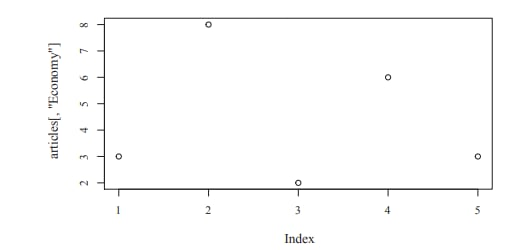
\includegraphics[width = \textwidth]{chapter/chapter2/figure2.8.jpg}
    \caption{The simplest X-Y plot.}
    \label{fig:placeholder9}
\end{figure}

\begin{figure}[!ht]
    \centering
    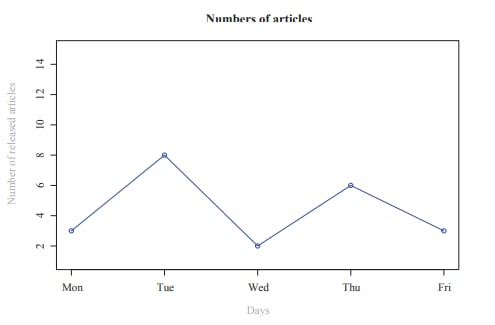
\includegraphics[width = \textwidth]{chapter/chapter2/figure2.9.jpg}
    \caption{A customized X-Y plot.}
    \label{fig:placeholder10}
\end{figure}

We can add another line for the articles from the \textit{Politics} category. It will
be red in color, the line will be dashed, and the points will be square in shape.
To clarify what is on the graph, a legend will be added. It will be placed on
a specified position in the graph (coordinates \cite{ref4,ref15}), the text will be slightly
smaller (the cex parameter), and the same line colors (the col parameter), point
types (the pch parameter), and line types (the lty parameter) used by the actual
plots will be used, see Figure 2.10).

\begin{figure}[!ht]
    \centering
    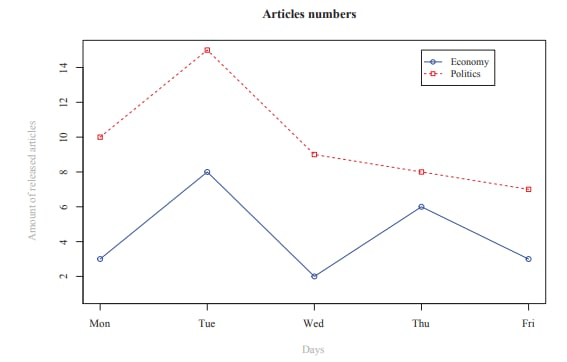
\includegraphics[width = \textwidth]{chapter/chapter2/figure2.10.jpg}
    \caption{A customized X-Y plot with two data segments.}
    \label{fig:placeholder11}
\end{figure}

\begin{figure}[!ht]
    \centering
    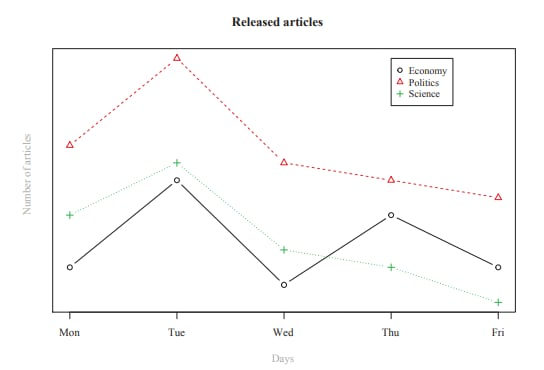
\includegraphics[width = \textwidth]{chapter/chapter2/figure2.11.jpg}
    \caption{A customized X-Y plot with three data segments.}
    \label{fig:placeholder12}
\end{figure}

\begin{verbatim}
> lines(articles[,"Politics"], type="o", pch=22,
+ lty=2, col="red")
> legend(4, 15, c("Economy","Politics"), cex=0.9,
+ col=c("blue", "red"), pch=21:22, lty=1:2)
\end{verbatim}

The \texttt{plot()} function is a good choice if you want to plot one or two columns
in one chart. When more data segments are to be displayed in a plot, another
function, \texttt{matplot()}, can be used instead (see Figure 2.11).

\begin{verbatim}
> matplot(articles, type ="b", pch=1:3, col=1:3,
+         axes=FALSE, ann=FALSE)
> title(main="Released articles")
> axis(1, at=1:5, lab=rownames(articles))
> axis(2, las=1, at=2*0:released_articles[2])
> box()
> title(xlab="Days", col.lab=’darkgrey’)
> title(ylab="Number of articles", col.lab=’darkgrey’)
> legend(4, 15, names(articles[1, ]), cex=0.9,
+        col=1:3, pch=1:3)
\end{verbatim}

A pie chart is a good option to show some proportions of a whole, for example, 
when we want to show how the newspaper articles in the \texttt{Economy} category are 
distributed in a week. This type of graph is created with the \texttt{pie()} function. 
The first parameter is a vector of non-negative numbers which are displayed as 
areas of pie slices. Other parameters include labels to be assigned to the slices, 
colors of the slices, or a title for the chart.

\begin{verbatim}
> colors <- c("green", "blue", "yellow", "orange", "red")
> pie(articles[, 1], main=names(articles[1, ])[1],
+     labels=names(articles[, 1]), col=colors)
\end{verbatim}

Slices with the specified colors, labeled with days are displayed in the chart
created. In the following example, we will add also the absolute numbers of
released articles together with the percentages rounded to one decimal place,
and a legend, see Figure 2.12).

\begin{verbatim}
> percent <- round(articles[, 1]/sum(articles[, 1]) * 100, 1)
> percent <- paste(percent, "%", sep="")
> pie(articles[, 1],
\end{verbatim}

\begin{figure}[!ht]
    \centering
    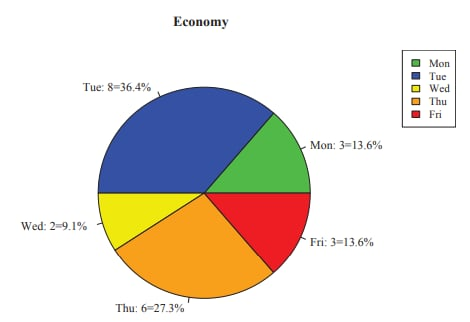
\includegraphics[width= \textwidth]{chapter/chapter2/figure2.12.jpg}
    \caption{Pie chart with labels and a legend.}
    \label{fig:placeholder13}
\end{figure}

\begin{figure}[!ht]
    \centering
    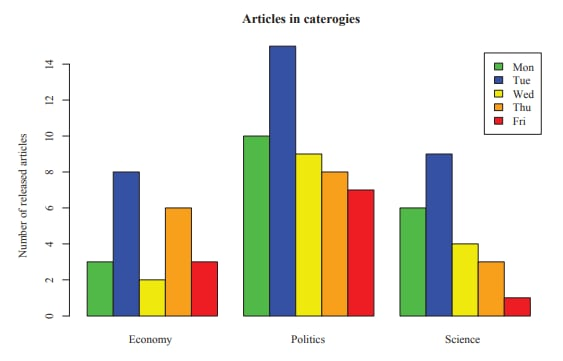
\includegraphics[width=\textwidth]{chapter/chapter2/figure2.13.jpg}
    \caption{Bar chart.}
    \label{fig:placeholder14}
\end{figure}

\begin{verbatim}
+ main=names(articles[1, ])[1],
+ col=colors,
+ labels=paste(paste(names(articles[, 1]),
+              articles[, 1],
+              sep=": "),
+              percent, sep="="))
> legend("topright", names(articles[, 1]),
+        cex=0.9, fill=colors)
\end{verbatim}  

A simple bar chart can be created using the \texttt{barplot()} function. 
If the first (or the \texttt{height}) parameter is a vector, 
a sequence of bars representing the numeric values of the vector will be created.

\begin{verbatim}
> barplot(articles[, 1])
\end{verbatim}

If the \texttt{height} parameter is a matrix, the bars correspond to the columns of
the matrix. The values in the columns are either stacked in one bar or represented
by a sequence of other bars (depending on the logical \texttt{beside} parameter). 
In our example, the x-axis will represent the newspaper categories and the sub-bars the
days of the week. The \texttt{t()} function can transpose the matrix so we can change
the perspective on the data (i.e., days on the x-axis and categories as sub-bars).

\begin{verbatim}
> barplot(articles)
> barplot(articles, beside=TRUE)
> barplot(t(articles))
\end{verbatim}

We can play with many parameters, for instance, adding descriptions of axes,
changing colors, or adding a legend.

\begin{verbatim}
> barplot(articles, main=’Articles in caterogies’,
+         ylab=’Number of released articles’,
+         beside=TRUE, col=colors, legend=TRUE)
\end{verbatim}  

We can customize many features of the graphical output through setting
graphical options using the \texttt{par()} function. This function, called without parameters,
returns a list of the values of current parameters. To change the parameters,
a list of \texttt{tag=value} pairs are submitted. The parameters include, for example,
justification of texts, margins, font, foreground or background colors, and many
others.














    












